\documentclass[10pt,a4paper]{article}
\usepackage{placeins}
\usepackage[utf8]{inputenc}
\usepackage[ruled]{algorithm2e}
\usepackage{fullpage}
\usepackage{graphicx}
\usepackage{float}
\usepackage[portuguese]{babel}
\usepackage[]{amsmath}
\restylefloat{figure}

\usepackage[adobe-utopia]{mathdesign}
\usepackage[T1]{fontenc}

% \usepackage{mdframed}

\DeclareGraphicsExtensions{.jpg,.pdf}

\numberwithin{equation}{section}

\title{Trabalho Prático 1 - Emulador}
\author{Victor Pires Diniz}

\begin{document}
\maketitle
\begin{center}
Software Básico - 2º Semestre de 2015
\end{center}

\section{Descrição do trabalho}

O primeiro trabalho prático do semestre propunha a implementação de um emulador que simulasse uma máquina virtual chamada ``Máquina de Khattab''. Esse programa deveria receber como entrada um programa em linguagem de máquina e emular sua execução, instrução a instrução.

\subsection{Detalhes sobre a Máquina de Khattab}

A máquina virtual se trata de uma arquitetura registrador-registrador (conhecida também como arquitetura \emph{load/store}) com instruções de no máximo dois operandos, que podem corresponder a registradores ou posições de memória, dependendo da instrução. Além dos 16 registradores de R0 a R15, há, também, alguns registradores de propósito específico:

\begin{itemize}
    \item \textbf{PC}: armazena posição atual a ser executada no programa. Modificado em instruções que alteram o fluxo de execução, como branches, jumps e chamadas a subrotinas.
    \item \textbf{PSW}: guarda informação sobre o resultado da última operação aritmética realizada, permitindo que instruções funcionem de maneira diferente se tal operação obteve resultado positivo, nulo ou negativo. (Útil para instruções de branch.)
    \item \textbf{SP}: mantém posição atual da pilha da máquina. Modificado em chamadas a subrotinas ou em instruções que empilham ou desempilham explicitamente.
\end{itemize}

A memória da máquina virtual tem pelo menos $1000$ posições capazes de armazenar um inteiro. Inteiros são a menos unidade endereçável e o único tipo de dados tratado pela MV. Além dos dados presentes no programa carregado, a máquina atua também na E/S padrão através de instruções de leitura e escrita. Programas são executados até encontrarem uma instrução \emph{HALT}, que indica o fim da execução.

\section{Implementação e decisões de projeto}

A fim de modularizar e garantir boa manutenibilidade, o código do emulador foi dividido em três módulos principais. O módulo \emph{Instr} lida com o comportamento de cada instrução, cada uma com sua própria função. Ele fornece, também, uma função que retorna, com base no \emph{opcode} de uma instrução, a função correspondente. \emph{Emulator}, por sua vez, define o comportamento e a estrutura da máquina virtual em si, permitindo instanciar um emulador, carregar um programa de um arquivo e executar a máquina. Finalmente, o arquivo \emph{main.c} apenas trata os parâmetros de execução em linha de comando e instancia o emulador. Por ser muito simples, não terá sua implementação analisada em mais detalhe, mas detalhes sobre os módulos restantes vêm a seguir.

\subsection{Instr}

Esse módulo é composto de dois arquivos. O header \emph{``instr.h''}, contém, além dos protótipos das funções acessíveis externamente, a definição de um \emph{enum} \emph{``instr''}, que pode assumir vários nomes diferentes que associam os \emph{opcodes} aos nomes mnemônicos das instruções, com a finalidade de melhorar a legibilidade do código.

O arquivo fonte \emph{``instr.c''} contém funções que desempenham a operação correspondente a cada instrução do conjunto de instruções definido na máquina virtual. Além dos operandos de cada instrução, essas funções recebem também como parâmetro uma referência ao emulador e seus atributos, permitindo acesso e modificação do banco de registradores, de posições na memória e dos registradores especiais.

Além disso, \emph{``instr.c''} define a função \emph{fetchInstr}, que recebe um \emph{opcode} como parâmetro e retorna a função correspondente à instrução. No entanto, em C, ponteiros de funções com protótipo diferente não são iguais, o que dificulta o retorno da função. Para contornar essa dificuldade, foi definido no header um \emph{union} chamado \emph{``oper''}, que contém um dos três tipos de função das instruções (zero, um ou dois operandos). Para permitir a decodificação do \emph{union}, o módulo define também um vetor que associa o opcode de cada instrução ao seu número de operandos.

\subsection{Emulator}

O módulo responsável pelo emulador da máquina virtual disponibiliza duas funções externamente no arquivo de \emph{headers} \emph{``emulator.h''}. \emph{``emuFromFile''} cria um novo emulador a partir de um arquivo de entrada, carregando o programa presente nesse arquivo para a memória. \emph{``emuRun''} inicializa o loop de execução do emulador, executando o programa carregado com os parâmetros especificados. Essa função permite, também, acionar o modo \emph{verbose}, que exibe informações de depuração para que o usuário possa avaliar se o programa está se comportando de acordo com o esperado.
Ainda nos \emph{headers} do módulo, é definido um \emph{struct} \emph{``emulator''}, que contém todos os elementos da máquina virtual: banco de registradores, memória etc. Também são declarados \emph{enums} para os modos de execução (simples e verboso) e para os três valores que o \emph{PSW} pode assumir (negativo, nulo e positivo).
O arquivo \emph{``emulator.c''} contém a implementação das funções do módulo. A função \emph{``runNext''}, presente nele, executa a próxima instrução no loop de execução da máquina virtual, apontada pelo contador de programa. Para isso, ela chama a função \emph{``fetchInstr''}, definida no módulo \emph{Instr}, e executa a instrução recebida de acordo com seu número de operandos. A função retorna o identificador da instrução executada, para que o loop de execução possa identificar a instrução ``HALT'' e interromper o fluxo do programa. As outras funções desse arquivo não são tão relevantes, e estão documentadas no próprio código fonte.

\section{Compilação e execução}

A compilação do emulador pode ser realizada através da \emph{makefile} disponibilizada ou diretamente através do \emph{GCC} ou outro compilador C. A execução do programa deve ser realizada através da linha de comando, na seguinte forma,

\begin{verbatim}
    {endereço do executável do emulador} <pc> <sp> <load_pos> <input> [output_mode]
\end{verbatim}

em que:

\begin{itemize}
    \item \verb|pc|: valor inicial do \textbf{PC} no emulador.
    \item \verb|sp|: valor inicial do \textbf{SP} no emulador.
    \item \verb|load_pos|: posição a partir do qual o programa de entrada será carregado na memória.
    \item \verb|input|: endereço para o arquivo de entrada, em linguagem de máquina.
    \item \verb|output_mode|: parâmetro \textbf{opcional} que permite escolher entre os modos de execução simples e verboso. Caso não seja especificado, o programa é executado em modo simples, sem informação de depuração. Valores válidos: \verb|s| (simples) ou \verb|v| (verboso).
\end{itemize}

\section{Testes realizados}

Na pasta de testes presente no pacote deste trabalho, há diversos programas que foram utilizados para garantir o bom funcionamento do emulador, cobrindo todas as instruções disponibilizadas pela especificação da máquina virtual. Segue abaixo uma breve descrição do comportamento de cada programa:

\begin{itemize}
    \item \verb|t_spec.i|: teste disponibilizado na especificação do trabalho, soma 100 a um número fornecido pelo usuário.
    \item \verb|t_fib.i|: calcula o número de Fibonacci de acordo com um índice fornecido pelo usuário.
    \item \verb|t_exp.i|: realiza a exponenciação de um número, de acordo com uma base e um expoente, ambos fornecidos pelo usuário.
    \item \verb|t_div.i|: realiza a divisão por força bruta de dois números inteiros, retornando quociente e resto.
    \item \verb|t_mdn.i|: determina a mediana de um conjunto de sete itens fornecidos pelo usuário.
\end{itemize}

O assembly correspondente a cada teste pode ser encontrado em uma pasta interna à pasta de testes.

\subsection{Imagens de execução dos testes}

\begin{figure}[h]
    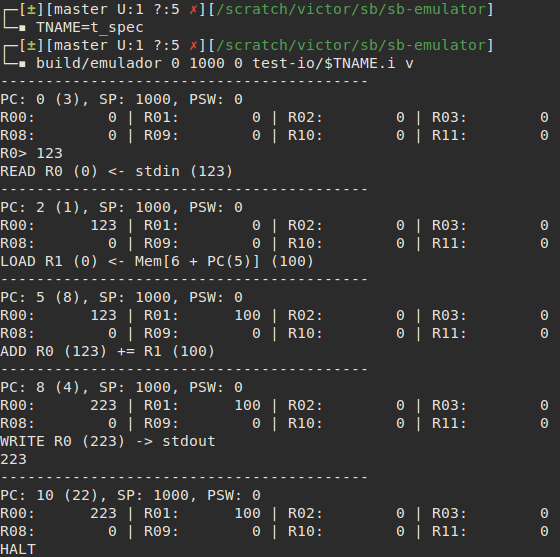
\includegraphics[scale=0.65]{imagens/t_spec_verbose_console.png}
    \centering
    \caption{Execução do teste t\_spec.i em modo verboso. Alguns registradores nulos não aparecem na imagem, para permitir melhor visualização.}
\end{figure}

\begin{figure}[h]
    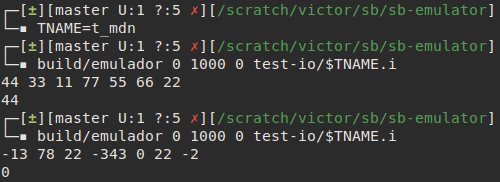
\includegraphics[scale=0.65]{imagens/t_med_console.png}
    \centering
    \caption{Execução do teste t\_mdn.i com dois conjuntos diferentes de entrada.}
\end{figure}

\begin{figure}[h]
    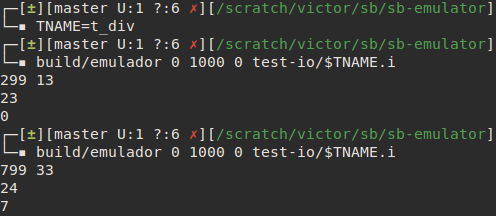
\includegraphics[scale=0.65]{imagens/t_div_console.png}
    \centering
    \caption{Execução do teste t\_div.i com dois pares diferentes de entrada.}
\end{figure}

\FloatBarrier

\section{Conclusão}

Neste trabalho, foi implementado um emulador para uma máquina virtual, definido de acordo com a especificação fornecida. O comportamento e a implementação do emulador foram discutidos no contexto dos testes realizados, de forma a garantir que as instruções funcionam como previsto.

\end{document}